\section{SRP-PHAT}
\subsection{Steered Response Power}
Steered Response Power (SRP) source localization is a method to detect sound source locations using beamforming techniques \cite{krim1996two}. SRP is different from TDOA based methods discussed before. While the generalized cross correlation is a simple cross correlation between each pair of microphones and only outputs an estimate of the time delay, the SRP method beamforms the space around the array and computes the energy of each location beam.  It `looks' at all possible directions individually (steering) and computes the power of the signal cross correlation in that direction (beamforming). The assumption is that the cross power of the steered microphone array will be the maximum in the correct source direction. However, the computational demand for this can rise quite fast (depending on the sampling rate and the angular resolution of the beamforming), making it nearly impossible to implement in real time applications. But, its performance in difficult conditions outperforms the TDOA based methods \cite{dmochowski2007generalized}. Since real-time localization is not of primary importance for this thesis, SRP based methods can be applied. In the same fashion as the GCC method proposed to pre-filter the signal before performing the cross correlation, a PHAT weighing can be applied on the beamformed signal. This method is called SRP-PHAT. %In this section, the first part discusses the basic principles behind the method whereas the second part introduces a hybrid method that improves the computational time of SRP without decreasing its robustness. 
The SRP method is based on a regular delay-and-sum beamformer, for a given point in space having range $\rho$, azimuth $\theta$ and elevation $\phi$ with the microphone array, the output of the beamformer is given by
\begin{equation}
    y_{\rho,\theta,\phi}(n)=\sum\limits_{m=0}^{M-1}{w_m x_m[n + f_{0,m}(\rho,\theta,\phi)]},
\end{equation}
where $x_0[n]$ is the signal received at time n, at an arbitrary microphone used as reference, $w_m$ is the amplitude weight for microphone m, and $f_{0,m}(\rho,\theta,\phi)$ is the relative delay between the reference microphone and the $m^{th}$ microphone. When far-field approximation is assumed, the range cannot be computed\footnote{For range computation, the cone approximation cannot be assumed. The delays should be used to compute hyperboloids and not cones. The intersection of the hyperboloids can then be used to compute range. However, it should be remembered that even a small error would lead to large variations in range, as for far-field, small movements in the hyperboloids would cause large movements in range results.} and the delay-and-sum beamformer output can be rewritten as follows:
\begin{equation}
    y_{\theta,\phi}(n)=\sum\limits_{m=0}^{M-1}{w_m x_m[n + f_{0,m}(\theta,\phi)]},
\end{equation}
For $w_m=1$ (assuming perfectly omni-directional and equally sensitive microphones), the output power of the beamformer becomes
\begin{equation}
    \mathbb{E}[{y_{\theta,\phi}(n)^2}]=\sum\limits_{i=0}^{M-1}\sum\limits_{j=0}^{M-1}{R_{x_i,x_j}[f_{i,j}(\theta,\phi)]} \text{, for } i\neq j.
    \label{eq:poweroutputbeamformer}
\end{equation}
This cross correlation is computed in the frequency domain (cross-spectrum) which is then inverse fast Fourier transformed (IFFT).
\begin{equation}
    R_{x_i,x_j}(\tau)= \sum\limits_{k=0}^{N_{f}-1}{X_{i}(k)X_{j}^*(k)e^{j2\pi\frac{k}{N_{f}}\tau}}
\end{equation}

Where $X_{i}(k)$ is the $N_{f}$ (number  point Fast Fourier Transform of a signal from the $i$ microphone.  

\subsection{Algorithm for SRP}
\begin{itemize}
    \item Compute the cross correlations of the signals received at all the microphone pairs. 
    \item Compute for each set of angles ($\phi,\theta$), the corresponding set of delays for every microphone pair $f_{i,j}(\theta,\phi)$. So if 1$\degree$ angular resolution is used, the SRP method computes delays for 360*180=64800 angular positions, for each microphone pair.
    \item For each ($\phi,\theta$), sum for all microphone pairs, the cross correlation values at the corresponding delays. This sum is the output of the SRP beamformer defined in Eq. \ref{eq:poweroutputbeamformer}\footnote{An improvement on the SRP search algorithm was proposed by pre-mapping the relative delays to their corresponding set of locations \cite{dmochowski2007generalized}. Instead of proceeding with a full sequential search in the 3D space, a search on the possible relative delays, where the cross correlation values are above a threshold, is considered. The possible delays between individual microphone pairs are already known based on the array geometry and can be stored in memory. The computational cost gain can be immense depending on the number of microphones. However, the method is not suitable if the whole acoustic map of an environment in required, so it is not detailed further here.}

%The cross correlations are calculated for each delay subset and related to a set of potential source location in space in the final steps of the algorithm. 
\end{itemize}
\begin{equation}
    S_{SRP}(\theta,\phi)=\sum\limits_{i=0}^{M-1}\sum\limits_{j=0}^{M-1}{R_{x_i,x_j}[f_{i,j}(\theta,\phi)]} \text{, for } i\neq j.\footnote{For a single source, the estimate of the source location from SRP search can be given by:
    $\hat{\phi},\hat{\theta}=\argmax_{\phi,\theta}S_{SRP}(\phi,\theta)$}
     \label{eq:srpSum}
\end{equation}
%\begin{figure}
%    \centering
%    \begin{subfigure}[t]{0.5\textwidth}
%    \centering
%    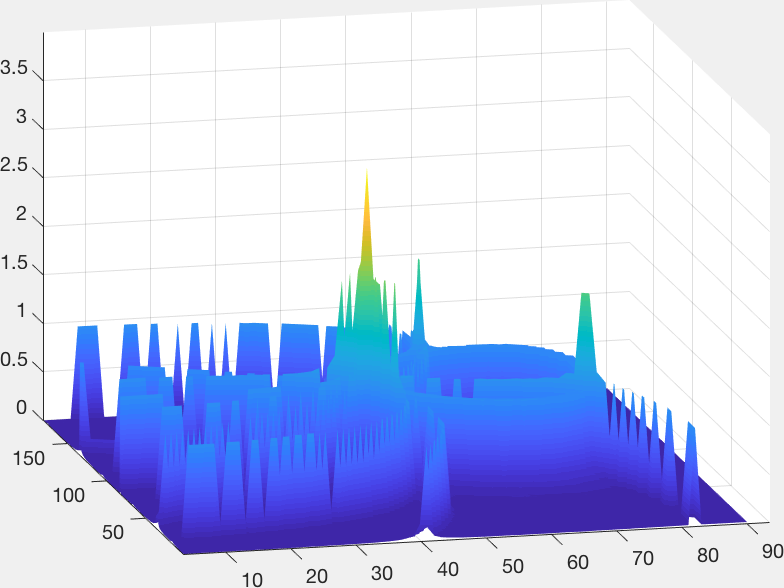
\includegraphics[width=0.9\textwidth]{Figures/viewside.png}
%    \caption{SRP map}
%    \label{fig:viewsidesrp}
%\end{subfigure}%
%\begin{subfigure}[t]{0.5\textwidth}
%    \centering
%    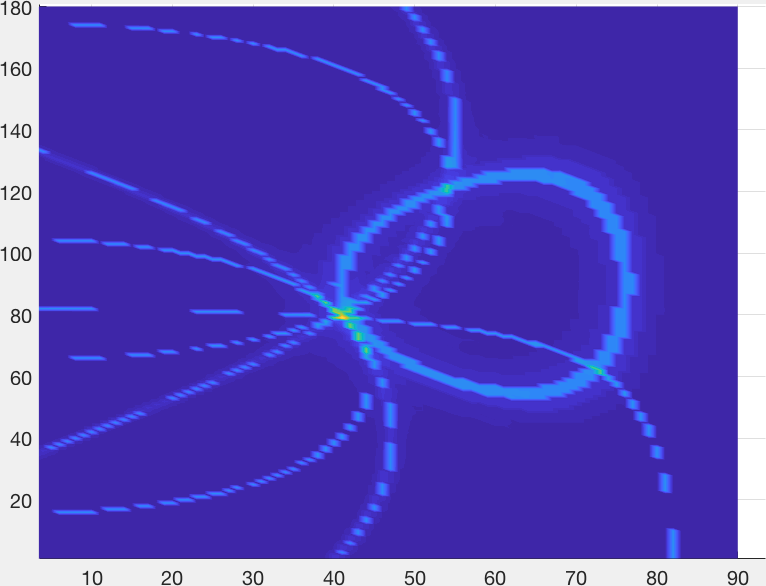
\includegraphics[width=0.9\textwidth]{Figures/topview.png}
%    \caption{SRP heat map}
%    \label{fig:topviewsrp}
%\end{subfigure}
%\caption{Power mapping simulation of source localized using SRP-PHAT algorithm in noiseless, free-field situation. For the simulation, first a 4-channel wav file is created such that the channels contain the same pink noise but delayed between each other. The delays are such that the source would be ideally located at azimuth $80\degree$ and elevation $40\degree$ when localized by a 1m aperture tetrahedral array. SRP-PHAT is then applied on the wav file and power received from different angles (beams) is computed and plotted. As can be seen the algorithm was able to localize the source in these ideal conditions fairly correctly.}
%\end{figure}
%The classical SRP search beamforms sequentially the 3D space and locations [($\phi_{1},\theta_{1}$), ($\phi_{2},\theta_{2}$), ... ,($\phi_{x},\theta_{x}$)] which might be associated with the same relative delay $\tau_{1}$ (in case of a uniform linear microphone array). The cross correlation at delay $\tau_{1}$ is then computed $x$ times, which leads to the same results for each [($\phi_{1},\theta_{1}$), ($\phi_{2},\theta_{2}$), ... ,($\phi_{x},\theta_{x}$)] positions, leading to numerous useless cross correlation computations.
%In GCC methods this issue was taken care of by interpolation, where the microphone pair end-side localization had poor resolution (Fig. \ref{fig:res_diff}). 
\subsection{Extending PHAT to SRP-PHAT}
PHAT can easily be extended to SRP-PHAT, by simply pre-filtering the cross-correlations before the SRP sum step,
\begin{equation}
    R_{x_i,x_j}(\tau)= \sum\limits_{k=0}^{N_{f}-1}{\psi_{ij}(k) X_{i}(k)X_{j}^*(k)e^{j2\pi\frac{k}{N_{f}}\tau}}
\end{equation}
where
\begin{equation}
    \psi_{ij}(k) = \frac{1}{|{X_{i}(k)X_{j}^*(k)}|}
\end{equation}
%Beamforming techniques for sound localization have been study intensively over the last decades. The main drawback of the conventional beamforming are the side lobes in the localization results. 
When localizing a point source using SRP-PHAT, the ideal result is to detect a point precisely at the actual point source location and nothing elsewhere. However that is not the case for SRP-PHAT. For instance, if two microphones are used, the only information that can be computed from localizing a single point source is the angle of incidence on the array. For a source located at (-50$\degree$, 60$\degree$)\footnote{For the purpose of this thesis, locations are designated as (x$\degree$, y$\degree$), signifying (azimuth, elevation) of the location respectively}, unsing two microphones located on the x axis (elevation $0\degree$) this leads to a circle (Fig. \ref{fig:2mic1src}) around the array where the source might be located. This is because the angle of incidence from every point on the circle, to the mid point of the line joining the two microphones, is the same. Thus, the circle is the base of the cone resulting from the cone approximation discussed before.
%For far-field, this means a plane wave incident with a particular DOA on the microphone array. In transfer function terms, the array response is `deconvolved' from the final energy map. 
%While this problem has motivated the creation of new beamformers {!!CITATION!!}, the problem lies in the method itself.
%New classes of algorithms have been developed to deconvolve the noise signals from the desired steered signal such as CLEAN \cite{sijtsma2007clean} and DAMAS \cite{brooks2006deconvolution}.
%DAMAS was acknowledged a major breakthrough in array processing. At first research was mainly focused on aeroacoustic for the development of near-field sound localization system but it seems that a new enthusiasm has taken over scientists trying to solve other sound localization problems. 
%While the DAMAS method is mainly designed for near field measurements in the range of the array aperture size, a new deconvolution method has been proposed [\cite{zhao2015large}, \cite{zhao2017large}] where a small aperture array is used to measure source signal in the far field. The principle behind point spread function is discussed in the following section. Then a review of the underlying principles of the main deconvolution algorithms is given, and finally a specific method for coherent and incoherent sources localization is discussed.

%\begin{figure}[H]
%    \centering
%    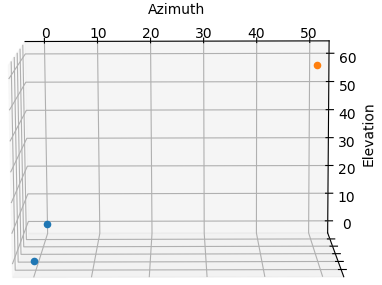
\includegraphics[width=0.98\textwidth]{Figures/2mic1src.png}
%    \caption{Figure depicts a source located at $50\degree$ azimuth and $60\degree$ elevation (orange dot). Two microphones (blue dots) will be used to localize the source.}
%    \label{fig:2mic1srcPos}
%\end{figure}
\begin{figure}[H]
    \centering
    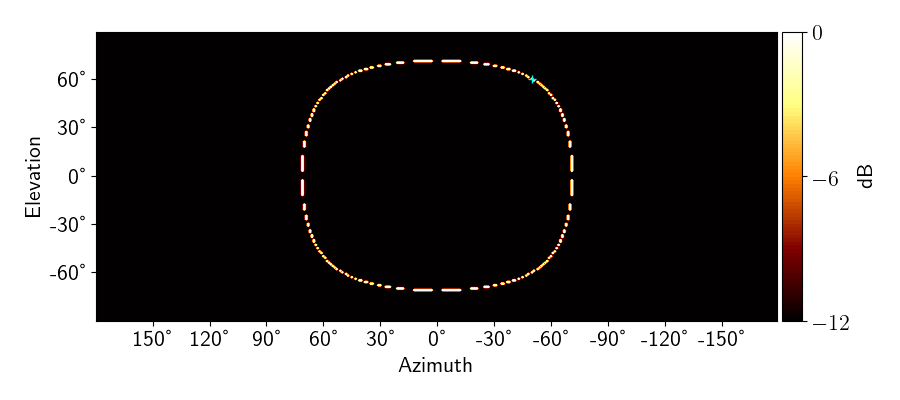
\includegraphics[width=0.8\textwidth]{Figures/2mic1srcRes.png}
    \caption{SRP-PHAT is run to localize a single point source using 2 microphones located on the x axis. The source can only be localized to a circle. The blue cross in the figure indicates the actual source location.}
    \label{fig:2mic1src}
\end{figure}
A new circle will result for each new microphone pair used to localize the source, for example, when using three microphones A, B and C placed in a horizontal equilateral triangle, three circles can be computed (one each for AB, BC and CA). The maximum peak occurs at 2 locations with (-50$\degree$,$\pm 60\degree$) as shown on figure \ref{fig:3mic1src}. For a tetrahedral array, 4 microphones are used and the array response is a combination of circles from the 6 possible microphone pairs ($^4C_2$). This time the main peak occurs at exactly one point. However, the cross-correlations values at computed delays are summed by the beamformer (Eq. \ref{eq:srpSum}) and subsidiary peaks can appear in the energy map at DOAs that don't correspond to the true source DOA, for example, points where only two of the circles meet. If multiple sources are localized, these peaks in the SRP-PHAT energy map can add up leading to the detection of a fake source or can mask real sources. Since only 3 pairs out of the 6 in a tetrahedral array are linearly independent (Eq. \ref{Eq:linearDep}), the localization can also be done considering only 3 of those pairs. The result in shown in fig. \ref{fig:4mic1srcInd}.
\begin{figure}[!ht]
    \centering
    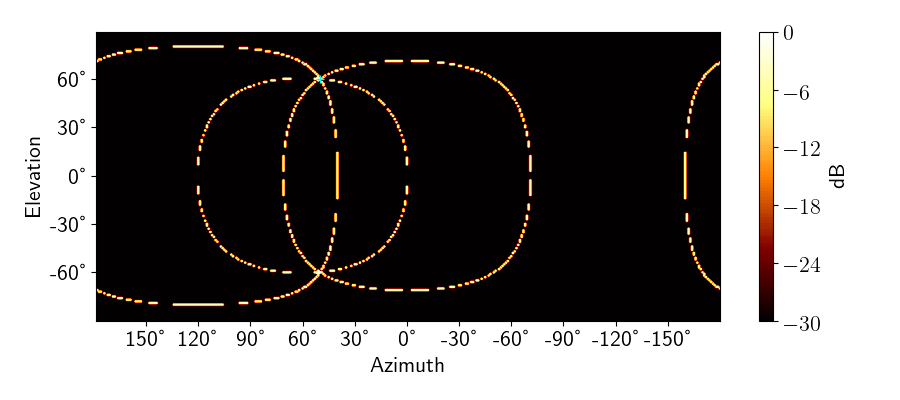
\includegraphics[width=0.8\textwidth]{Figures/3mic1srcRes.png}
    \caption{SRP-PHAT is run to localize the source with 3 microphones.}
    \label{fig:3mic1src}
\end{figure}
\begin{figure}[!ht]
    \centering
    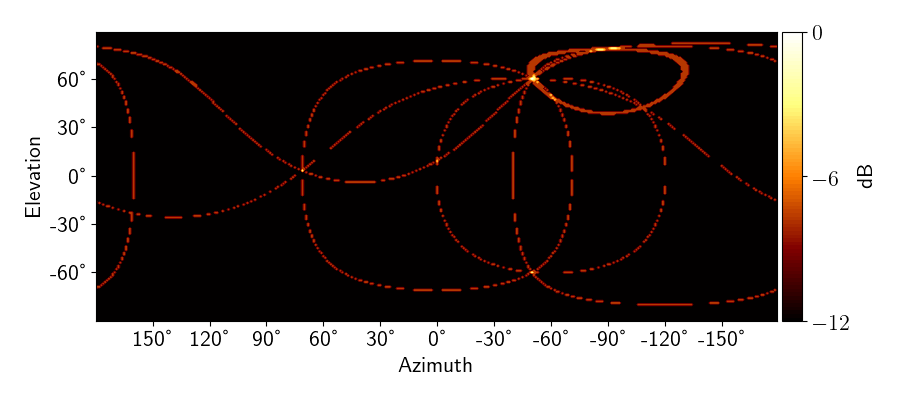
\includegraphics[width=0.8\textwidth]{Figures/4mic1srcRes.png}
    \caption{SRP-PHAT is run to localize the source with a tetrahedral array.}
    \label{fig:4mic1src}
\end{figure}
\begin{figure}[!ht]
    \centering
    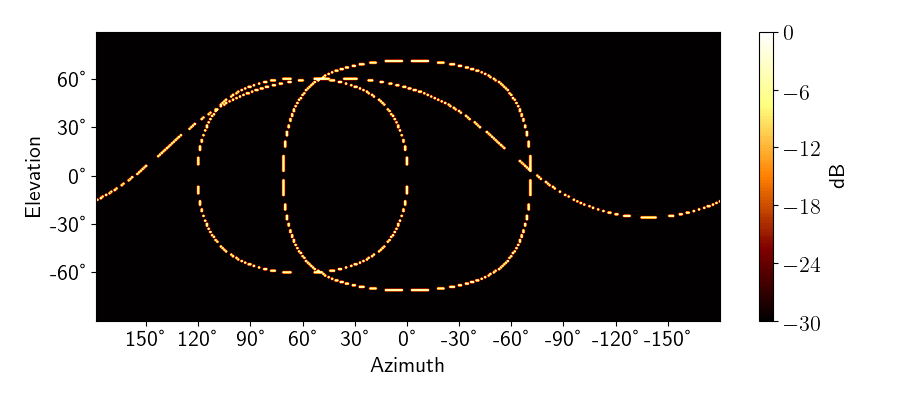
\includegraphics[width=0.8\textwidth]{Figures/Ind4mic1srcRes.png}
    \caption{SRP-PHAT is run to localize the source with a tetrahedral array but only linearly independent microphone pairs are considered}
    \label{fig:4mic1srcInd}
\end{figure}
Considering only independent microphones, Eq. \ref{eq:srpSum} can be rewritten as,
\begin{equation}
    S_{SRP}(\theta,\phi)=\sum\limits_{i=1}^{M-1}{R_{x_0,x_i}[f_{0,i}(\theta,\phi)]}
     \label{eq:srpSumInd}
\end{equation}
%\subsection{Using the redundant information from the microphone pairs}
The thing to note is that Eq. \ref{Eq:linearDep} is only true for no noise conditions. In noisy conditions, there is a potential to gain information by using the redundant microphone pairs. This is because if noise at all microphones is assumed to be uncorrelated, then even if the noise causes certain microphone pairs to detect a source at a `sourceless' location, other microphone pairs might have a lower magnitude at that location. Due to more microphone pairs, the sum of all microphone pairs will be even higher at the real source location, and at other locations, the sum due to the noise will be suppressed. It can be seen in Fig. \ref{fig:4mic1src} that using all the microphone pairs adds to the overall noise on the map as more pairs can now contribute to the SRP sum, leading to more circles. However, ideally, the peak of the true source would also become higher, due to more pairs providing power at the source location. This can means that even though the noisy floor is has noise in more locations, it is less noisy, leading to a better dynamic range. For this reason, for the rest of this thesis, all possible pair of microphones are considered for localizing.
%\begin{figure}[H]
%\begin{subfigure}[b]{0.96\textwidth}
%    \centering
%    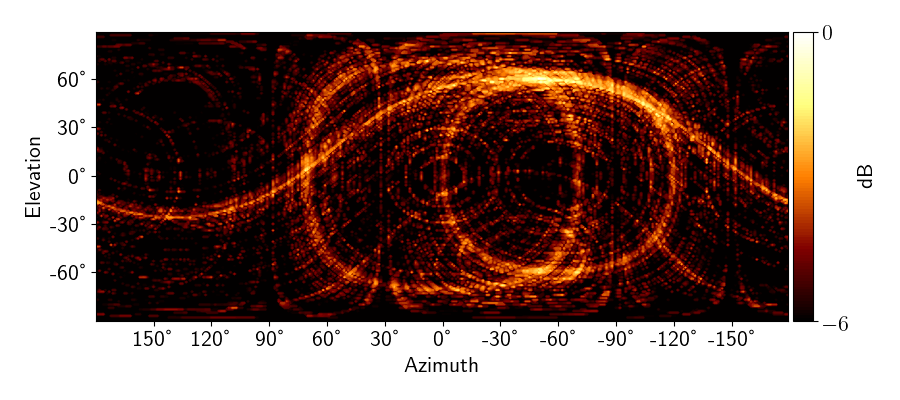
\includegraphics[width=0.8\textwidth]{Figures/Ind4mic1srcResNeg10LowDyn.png}
%\end{subfigure}
%\vskip \baselineskip
%\begin{subfigure}[b]{0.96\textwidth}
%    \centering
%    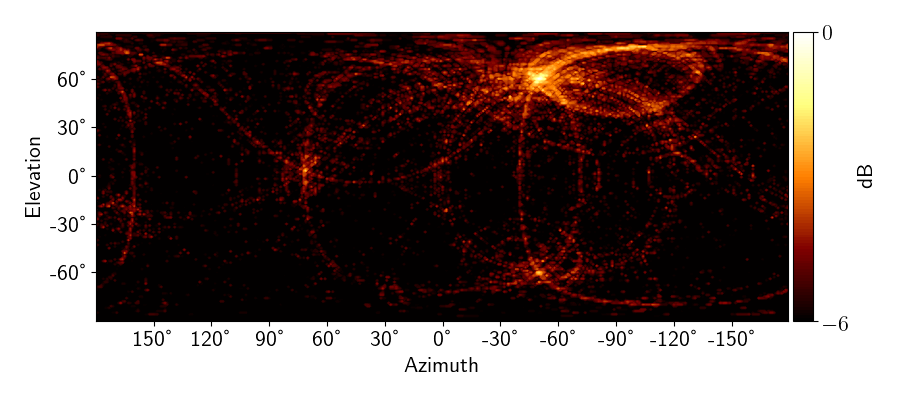
\includegraphics[width=0.8\textwidth]{Figures/Dep4mic1srcResNeg10LowDyn.png}
%\end{subfigure}
%\caption{Figures depict from SRP-PHAT localization results with SNR = -10dB, for independent microphone pairs (top), and for all  microphone pairs (bottom)}
%\label{fig:4mic1srcRedun}
%\end{figure}
%\subsubsection{Simulations}
%Two identical sound sources are placed in the far field. A tetrahedral array with equal spacing between microphones of 1 meter is receiving the two sources. The sound received at the sources are 3 seconds of two different pink noises with respective DOA $\tetha_{1}=120\degree$, $\phi_{1}=40\degree $ and $\tetha_{2}=150\degree $ , $\phi_{2}=75\degree $. Waves are propagating in free field where no reflections and no noise is added to the microphones. The SRP maps are computed and displayed in the figure \ref{fig:coherent2pinknoise}. Source 2 is placed at a problematic angle for the tetrahedral array, detection errors are discussed in section \ref{sec:detection}. Error probability increases as the source DOA approach the angle of the axis drawn by pairs of microphones (end-side).
%\begin{figure}[H]
%    \centering
%    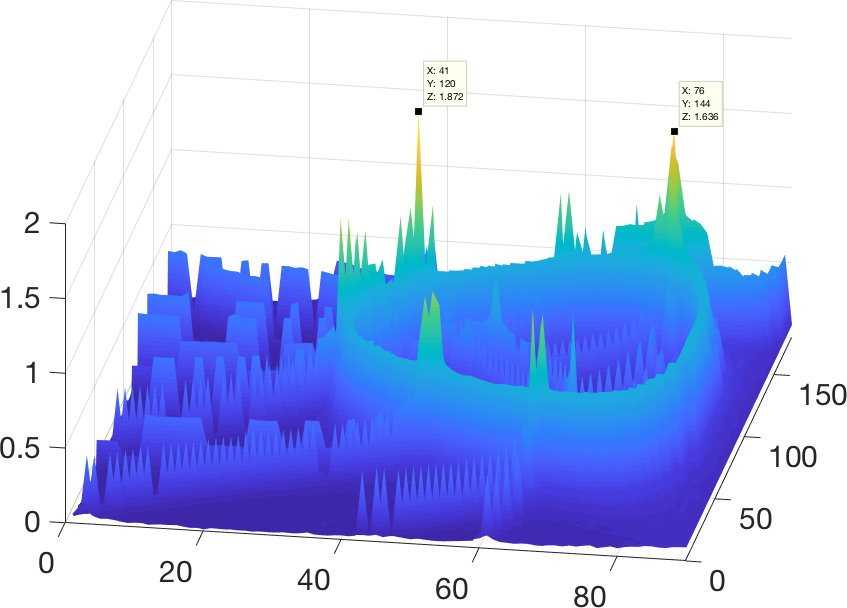
\includegraphics[width=1\textwidth]{Figures/2pinknoisesrpphat.png}
%    \caption{SRP-PHAT simulation with 2 sound sources localized using a tetrahedral array}
%    \label{fig:coherent2pinknoise}
%\end{figure}
%\subsubsection{Localization errors} \label{sec:detection}
%Two pairs of microphones are considered, the axes drawn by the two pairs is plotted (extended) in figure \ref{fig:locerrortetra}. The two axes form respective angles of $45\degree$ and $60\degree$ with the horizontal axis. Plane waves with DOA between $45\degree$ and $60\degree$ will cross the two pairs of microphones at an angle close to the respective end-sides of the pairs. As shown in figure \ref{fig:errorsimulation1} maximum errors arise in the simulation for DOA contained in between $45\degree$ and $60\degree$. For a tetrahedral array, this can be seen as the 3d space created by extending the arms connecting the microphones. 
%\begin{figure}[H]
%    \centering
%    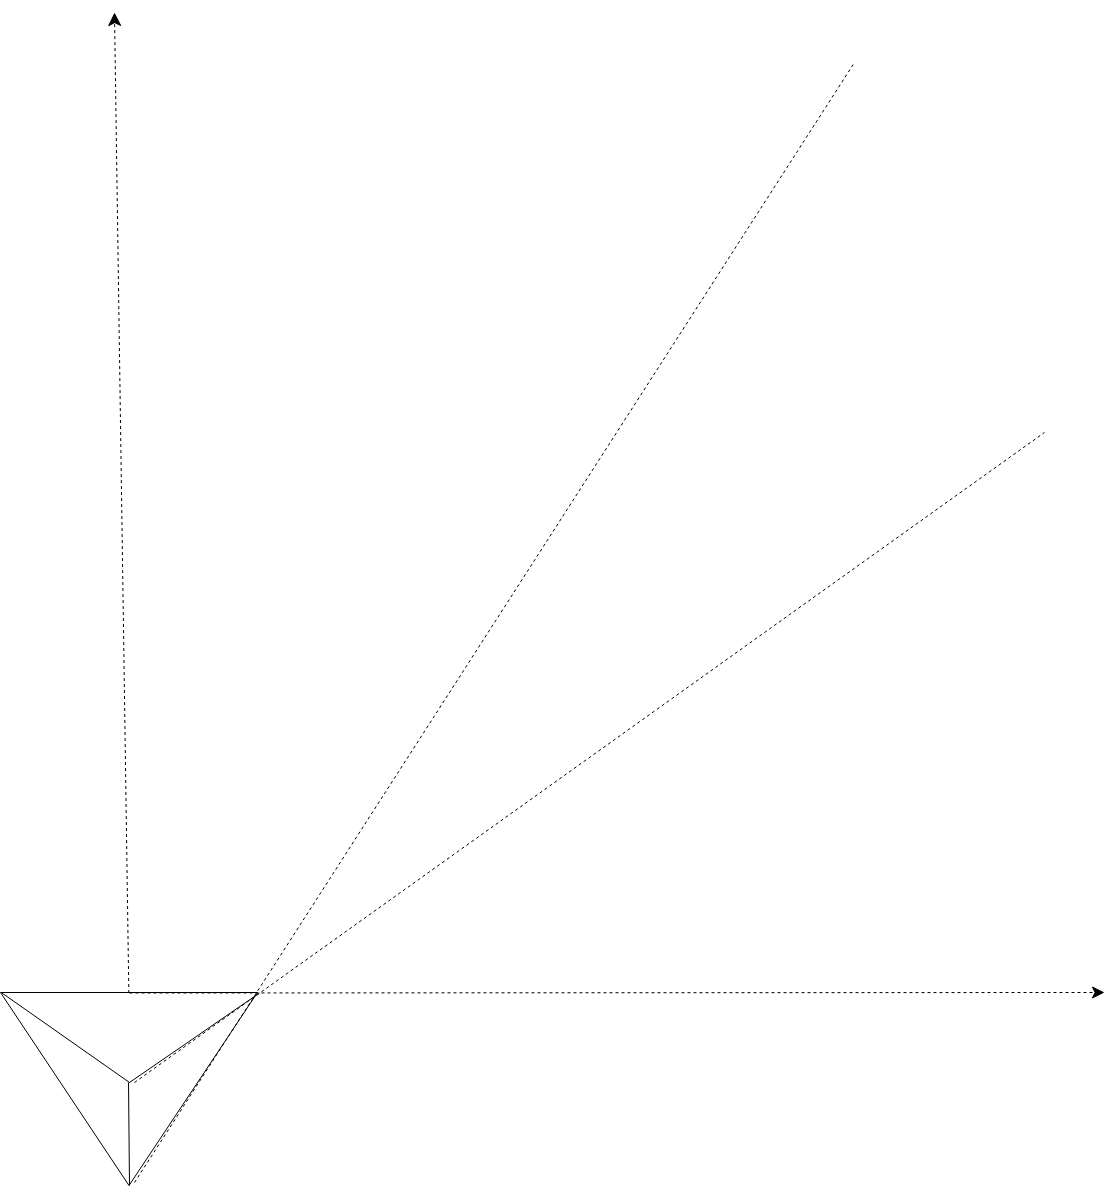
\includegraphics[width=0.9\textwidth]{Figures/locerrors.png}
%    \caption{Axis drawn by 2 pairs of microphones}
%    \label{fig:locerrortetra}
%\end{figure}
%\begin{figure}[H]
%    \centering
%    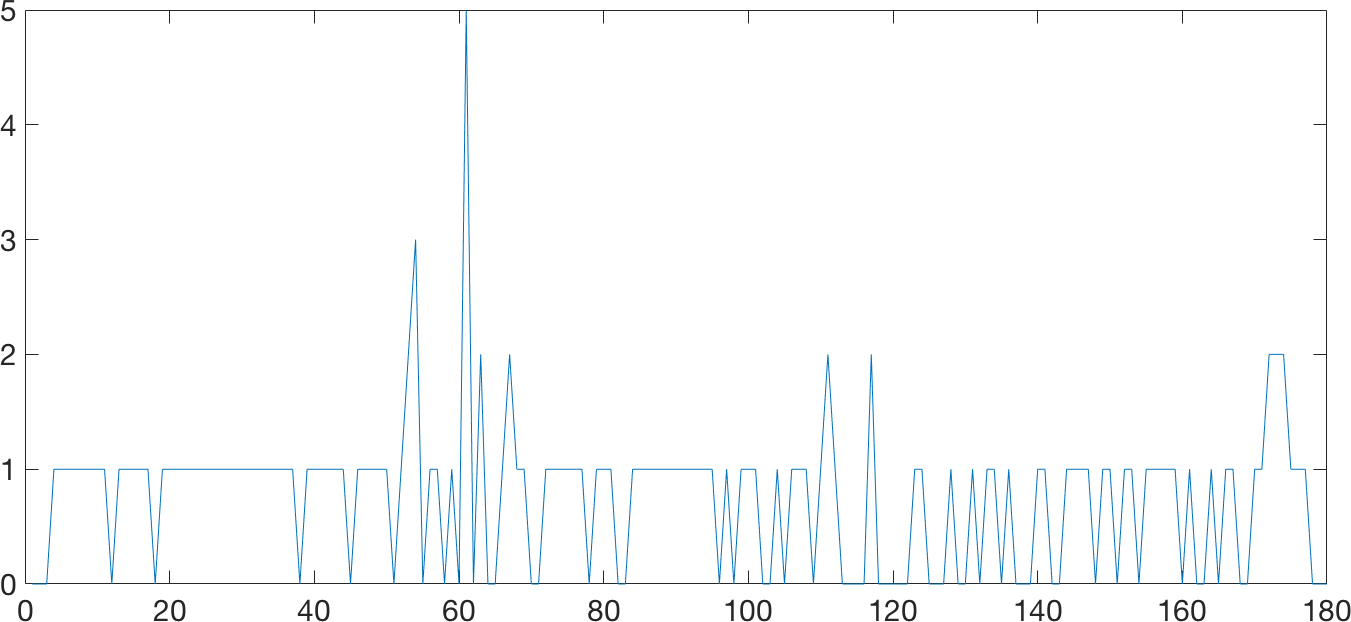
\includegraphics[width=0.9\textwidth]{Figures/errorphinointerpolationandrounding.png}
%    \caption{Simulation errors with no interpolation}
%    \label{fig:errorsimulation1}
%\end{figure}
%\subsubsection{Temperature and noise}
%Temperature is a major parameter of the algorithm and it affects the speed of sound in air and ultimately the propagation delay in the array.
%\subsubsection{SRP vs SRP PHAT}
%An experiment is design to test our implementations of SRP and SRP PHAT. A prototype tetrahedral microphone array is placed outside, the ideal free field condition are not holding since ground effect and reflections from the nearby buildings will affect the sound waves received by the array. The SNR cannot be controlled and is found to be, 

